\section{PCA analysis}
\subsection{PCA and projections}
\noindent
We decided to perform a PCA analysis in order to improve the performance of our
linear model. After performing a Single Value Decomposition, we want to detect which
which regressor mstly related to noise we have to include in our design matrix. Below
the projection of the brain data onto the new basis U.

\begin{figure}[H]
    \centering
        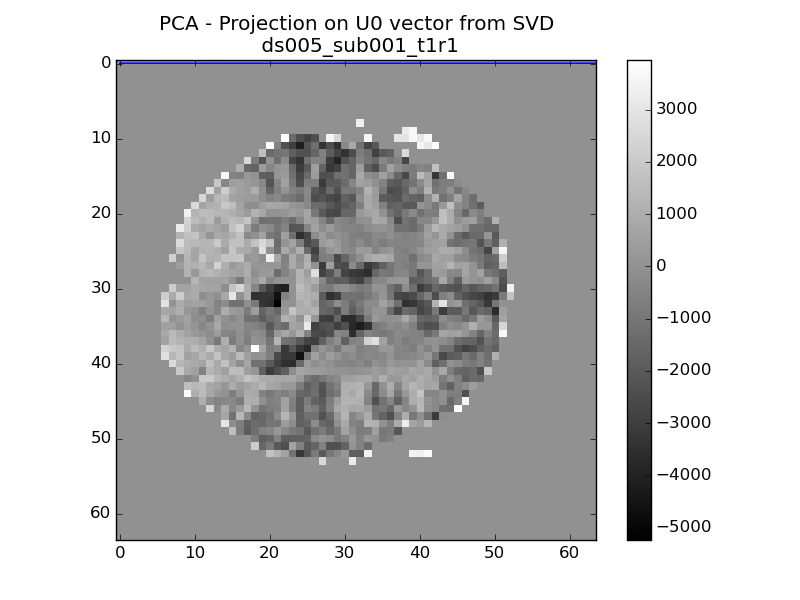
\includegraphics[scale=0.5]{../plots/ds005_sub001_t1r1_projection_U0.png}
     \caption{Brain data projected onto the new basis U - projection on U0 - subject 1 - run 1}
\end{figure}

\begin{figure}[H]
    \centering
        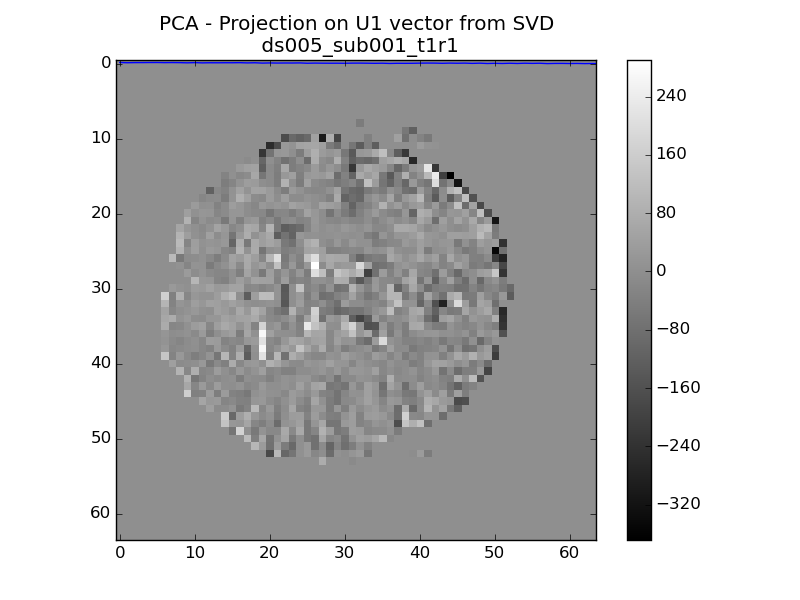
\includegraphics[scale=0.5]{../plots/ds005_sub001_t1r1_projection_U1.png}
     \caption{Brain data projected onto the new basis U - projection on U1 - subject 1 - run 1}
\end{figure}

\noindent
The two images above, show that strong localization of the voxels at the edges of the
brain, which suggests that they reflect brain anatomy rather than activation. 
We decided to remove these components by regression because they are likely to be 
related to noise from the scanner or the subject. 

\begin{figure}[H]
    \centering
        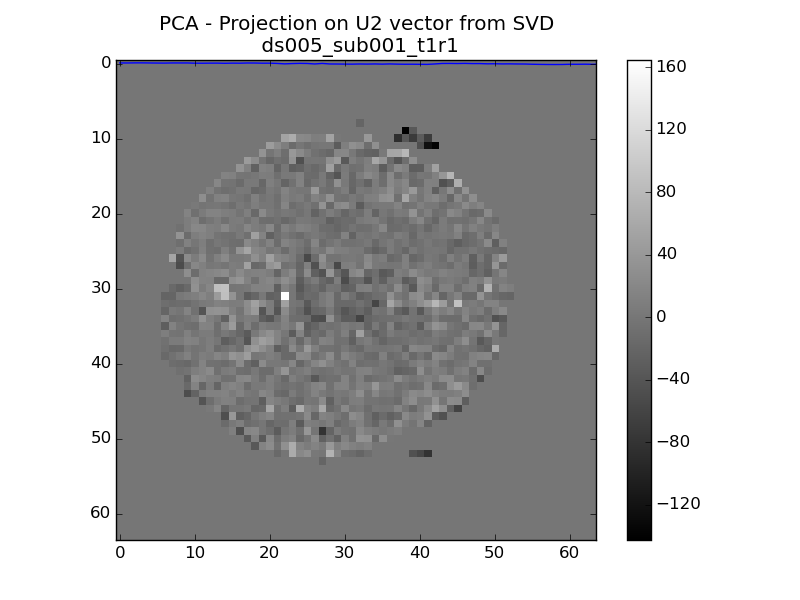
\includegraphics[scale=0.5]{../plots/ds005_sub001_t1r1_projection_U2.png}
     \caption{Brain data projected onto the new basis U - projection on U2 - subject1 - run 1}
\end{figure}

\begin{figure}[H]
    \centering
        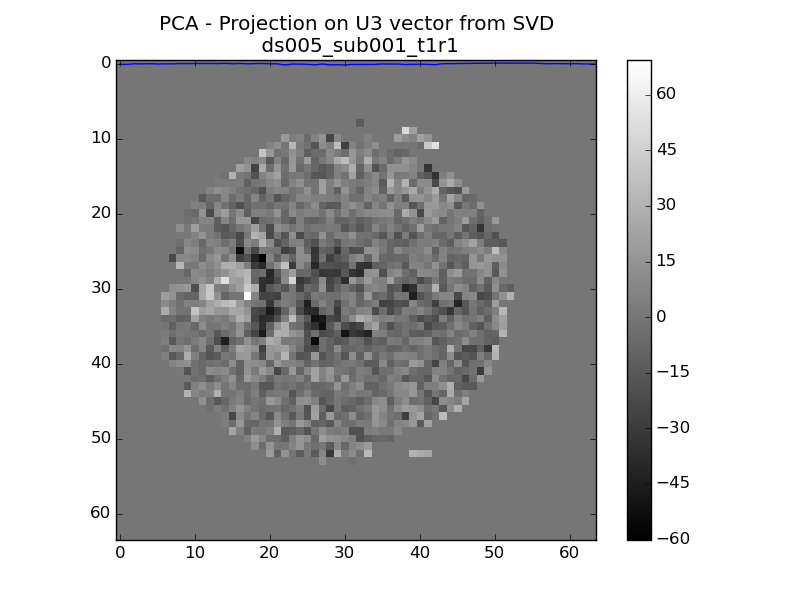
\includegraphics[scale=0.5]{../plots/ds005_sub001_t1r1_projection_U3.png}
     \caption{Brain data projected onto the new basis U - projection on U3 - subject 1 - run 1}
\end{figure}

\noindent
Contrary to the precedent cases, the above two images of the projection of th 3rd and
4th component don't seem to reveal any random pattern. The projection on the 4th 
component show a darker area localized on the startium.
In order to determine how many more components to remove from the analysis, we plotted 
the following Variance Explained plot.
\noindent
In the Single Value Decomposition, the vector S contains the square roots of the 
singular values ordered from greatest to least along its diagonal. Each value 
indicates the variance of the component vector (time-course) along each dimension 
of U. 
\noindent
In the figure below, each elements of the matrix S has been normalized. We decided 
to remove the first component from the graph for better clarity.
The first principal component accounts for 98 percent of the overall variability,
the second explains for 0.03percent.
In this particular case, removing the first principan component from the regression
makes the more sense, which is a bit different from our previous intuition that
considered the first two.

\begin{figure}[H]
    \centering
        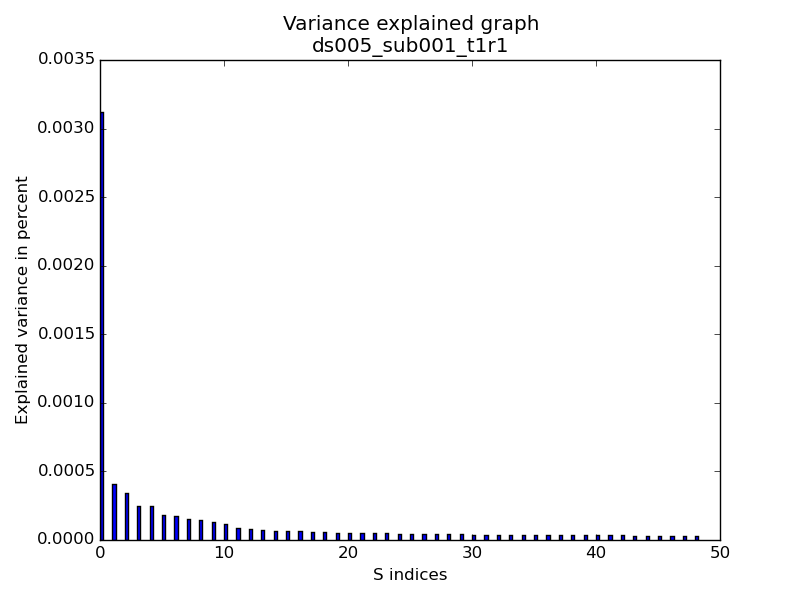
\includegraphics[scale=0.4]{../plots/ds005_sub001_t1r1_variance_explained.png}
     \caption{Variance explained for the subject 1 - run 1 (first term remove for clarity of the graph)}
\end{figure}

\noindent
After including the first principal component in our design matrix, we perform our
linear regression again and a new design matrix. The mean residual sum of square 
did not different much before and after the PCA analysis. Before the PCA analysis, 
the mean of the MRSS is 95.9, after it decreases to 94.6 for this particular subject 
and this particular run.

\subsection{Next steps}
\noindent
We need to extend the study accross all subjects of the experiments and we want to
validate our model accross runs for the same subject.
We find difficulties in validating our model for the same subject with a different
run. The challenge comes from the fact that the mask applied to determine which
voxels are inside the brain change the dimension of our data.


